\documentclass[twoside,a4paper,12pt]{article}
\hfuzz=5pt
\usepackage{textcomp} % Additional symbols and better font compatibility

% Packages
\usepackage[a4paper,margin=1in]{geometry} % A4 layout

\usepackage{amsmath,amsfonts,amssymb} % For math formatting
\usepackage{minted} % For syntax highlighting
\usepackage{titlesec} % For custom section formatting
\usepackage{xcolor} % For color definitions
\usepackage{fontspec}
\usepackage{unicode-math}
\usepackage{newunicodechar}
\definecolor{myDarkBlue}{HTML}{0b077d}
\definecolor{emerald}{HTML}{005945}
\usepackage[hidelinks, colorlinks=true, citecolor=emerald, urlcolor=myDarkBlue, linkcolor=emerald, linktoc=all]{hyperref}
\renewcommand{\chapterautorefname}{Chapter}
\renewcommand{\sectionautorefname}{Section}
\renewcommand{\figureautorefname}{Figure}
\renewcommand{\subsectionautorefname}{Section}
\usepackage{booktabs} % For better table formatting
\usepackage{graphicx}

\usepackage[style=nature, maxbibnames=3, doi=false, url=false, isbn=false, hyperref=true, backref=true, natbib=true, labelnumber]{biblatex}
\DefineBibliographyStrings{english}{%
    backrefpage = {Page},% originally "cited on page"
    backrefpages = {Pages},% originally "cited on pages"
}
\addbibresource{bib.bib} % Replace with your .bib file
\renewcommand\bfdefault{b}  % Ensure bold text
\renewcommand\itdefault{it} % Ensure italic text

\fvset{fontfamily=tt}
\newcommand{\setmonofontblock}{\setmonofont{LigaSFMonoNerdFont-SemiBold}}
\newcommand{\resetmonofont}{\setmonofont{Latin Modern Mono}}
\setmonofont{Latin Modern Mono}

\renewcommand{\theFancyVerbLine}{\sffamily \textcolor[rgb]{0,0,0}{\tiny \oldstylenums{\arabic{FancyVerbLine}}}}

\definecolor{bg}{HTML}{282C34}


% Title formatting
\titleformat{\section}{\large\bfseries}{\thesection}{1em}{}
\titleformat{\subsection}{\normalsize\bfseries}{\thesubsection}{1em}{}

\usepackage{fancyhdr} % For custom headers and footers
\pagestyle{fancy}

% Clear all default header and footer fields
\fancyhf{}

% Footer with page numbering
\fancyfoot[C]{Page \textbf{\thepage} of \textbf{\hypersetup{linkcolor=black}\pageref{LastPage}\hypersetup{linkcolor=emerald}}}

% Conditional header for "faa42"
\fancyhead[LE,RO]{\textsl{faa42}} % Left on odd pages, right on even pages
\fancyhead[LO,RE]{}      % Clear conflicting fields
\fancypagestyle{plain}{  % Define style for the first page
  \fancyhf{}             % Clear headers and footers
  \renewcommand{\headrulewidth}{0pt} % Remove header line
}
\renewcommand{\headrulewidth}{0.4pt} % Add header rule for other pages
\setlength{\headheight}{14.5pt} % Adjust the header height
\addtolength{\topmargin}{-2.5pt} % Compensate for the increased header height

% Extra package to determine total page count
\usepackage{lastpage}


% Document Title Page
\title{\textbf{Cryptography and Protocol Engineering (P79)\\ Assignment 2}}
\author{Firas Aleem \textsl{(faa42)}}
\date{Lent 2024 \\\vspace{0.5cm} {\small Word Count: 2,047}\footnote{Word count excludes code listings and appendices.}}

\begin{document}
%TC:ignore

% Title Page
\maketitle
\thispagestyle{empty}
\newpage

\newcommand{\smalltt}[1]{\texttt{\small #1}}

%TC:endignore

% Main Content Heading
% --- 1. INTRODUCTION ---
\section*{Assignment 2: SIGMA and SPAKE2 Protocols}
\label{sec:introduction}

This report details the implementation of the SIGMA and SPAKE2 protocols using X25519 and Ed25519 for secure key exchange and authentication. SIGMA enables authenticated key exchange with certificates, while SPAKE2 facilitates password-authenticated key exchange (PAKE) without a public key infrastructure. \\

A key focus of this assignment was designing a structured and consistent cryptographic API. Initially, my X25519 and Ed25519 implementations from Assignment 1 \cite{aleem2024curve25519} handled raw 32-byte keys, which raised usability and security concerns. As I integrated them into SIGMA and SPAKE2, I refined my API to ensure consistency, usability, and correctness.

The report is structured as follows:
\begin{itemize}
\item \textbf{\autoref{sec:api_refactoring}} discusses API refactoring for X25519 and Ed25519, highlighting key improvements.
\item \textbf{\autoref{sec:sigma}} explains the SIGMA protocol, including certificate authority (CA) design and secure messaging.
\item \textbf{\autoref{sec:spake2}} presents the SPAKE2 implementation and its security considerations.
\item \textbf{\autoref{sec:future}} explores potential extensions and optimizations.
\end{itemize}

This project reinforced the importance of practical, well-structured cryptographic code. Iterative improvements led to a more robust and maintainable implementation.

% --- 2. API DESIGN AND REFACTORING ---
\section{Refactoring the Cryptographic API}
\label{sec:api_refactoring}

% Discussing the original approach and why refactoring was necessary.
In my initial implementation for Assignment 1, cryptographic keys were handled as raw 32-byte values. While functional, this approach had drawbacks:

\begin{itemize}
    \item \textbf{Security Risks}: Storing private keys as raw byte arrays increased the risk of accidental exposure.
    \item \textbf{Lack of Structure}: Without a defined key abstraction, operations like key exchange and signing required manual byte management.
\end{itemize}

To address these issues, I introduced structured key classes for \texttt{X25519} and \texttt{Ed25519}, encapsulating key-related operations within dedicated objects.

\subsection{Ensuring Consistency in API Design}
\label{subsec:api_consistency}

While adding key classes improved structure, inconsistencies emerged when integrating them into the SIGMA and SPAKE2 protocols. For example:
\begin{itemize}
    \item \texttt{Ed25519} had a method \texttt{signingKey.generate\_verifying\_key()}, while
    \item \texttt{X25519} required calling \texttt{X25519PublicKey.from\_private\_key()}.
\end{itemize}
This inconsistency complicated API usage by requiring different function calls for similar operations. To fix this, I aligned their methods so that public or verifying keys could always be derived from their corresponding private or signing keys.

To refine the design further, I did the following:
\begin{itemize}
    \item \texttt{exchange()} for X25519 to handle Diffie-Hellman key exchange.
    \item \texttt{sign()} and \texttt{verify()} for Ed25519, eliminating the need for manual instantiation.
\end{itemize}

These improvements simplified cryptographic operations and enhanced API usability.\footnote{After refactoring, all test cases ran successfully (see the \texttt{tests\_ass1} folder).} \\

\textbf{Lessons Learned:}
\begin{itemize}
    \item Designing an API without using it in real-world scenarios led to usability issues that became evident during SIGMA and SPAKE2 integration.
    \item Maintaining consistency across cryptographic primitives is crucial for usability and maintainability.
\end{itemize}

This refactoring ultimately resulted in a cleaner, more intuitive cryptographic API, making protocol implementation significantly smoother.

% --- 3. SIGMA PROTOCOL ---
\usemintedstyle[python]{one-dark, linenos, breaklines, bgcolor=white, framesep=3mm, baselinestretch=1.2, firstnumber=last, fontsize=\footnotesize}

\section{Implementing the SIGMA Protocol}
\label{sec:sigma}

\subsection{Designing the SIGMA Protocol}
\label{subsec:sigma_design}

My implementation of the SIGMA protocol follows the lecture notes \cite{P79LectureNotes} and Section 5.1 of Krawczyk's SIGMA paper \cite{SIGMA}. The protocol establishes a secure session between two parties, Alice and Bob, by combining:

\begin{itemize}
\item \textbf{Key exchange} (X25519) to derive a shared secret.
\item \textbf{Authentication} (Ed25519) to sign ephemeral keys and verify identities.
\item \textbf{Message integrity} (HMAC-SHA256) to ensure authenticity.
\end{itemize}

The handshake consists of four steps across three message exchanges:

\begin{enumerate}
\item \textbf{Initiator (Alice)} sends her ephemeral public key.
\item \textbf{Responder (Bob)} responds with his ephemeral key, certificate, and signature.
\item \textbf{Initiator} verifies Bob's response, signs the keys, and sends her certificate.
\item \textbf{Responder} verifies Alice's identity and finalizes the session.
\end{enumerate}

To ensure modularity and maintainability, I structured the implementation into four key classes:

\begin{enumerate}
\item \mintinline{python}{SigmaParty} - Manages key pairs and certificates for Alice and Bob.
\item \mintinline{python}{SigmaHandshake} - Orchestrates the handshake, handling key exchange and authentication.
\item \mintinline{python}{SigmaKeys} - Derives session and authentication keys using HKDF.
\item \mintinline{python}{SecureChannel} - Provides encrypted messaging after the handshake via AES-GCM.
\end{enumerate}

This modular approach improves testability, extensibility, and debugging.

\subsection{SigmaKeys: Derivation and Security Considerations}
\label{subsec:sigma_keys}

The \mintinline{python}{SigmaKeys} class derives session and authentication keys from the shared secret. Instead of hashing the shared secret with domain separation strings (as in the lecture notes), I used HKDF for stronger key separation and security.

\begin{itemize}
    \item \textbf{HKDF for Key Separation:} Ensures independent keys for session encryption ($k_S$) and message authentication ($k_M$), even if the shared secret is reused.
    \item \textbf{Improved Domain Separation:} Longer separation strings further reduce key collision risks.
    \item \textbf{AES-GCM for Encryption:} Similar to TLS cipher suites (e.g., \mintinline{python}{TLS_AES_128_GCM_SHA256}) but uses 256-bit keys for stronger security.
    \item \textbf{Redundant HMAC-SHA256:} Initially added despite AES-GCM's built-in authentication. Benchmarks showed negligible overhead, so I retained it as an additional integrity check.
\end{itemize}


\subsection{Certificate and CA Design}
\label{subsec:sigma_ca}

To simplify implementation, I used a minimal JSON-based certificate format instead of X.509:

\usemintedstyle[json]{one-dark, linenos, breaklines, bgcolor=bg, framesep=4mm, baselinestretch=1.2, firstnumber=last, fontsize=\footnotesize}

%TC:ignore
\setmonofontblock
\begin{minted}{json}
{
    "subject_name": "Alice",
    "subject_key_b64": "<base64-encoded key>",
    "issuer_name": "TestCA",
    "signature_b64": "<base64-encoded signature>"
}
\end{minted}
\resetmonofont
%TC:endignore

\usemintedstyle[json]{one-dark, linenos, breaklines, bgcolor=white, framesep=3mm, baselinestretch=1.2, firstnumber=last, fontsize=\footnotesize}

This approach avoids unnecessary complexity in the implementation and implements the key features needed in a certificate, such as the subject's name, public key, issuer, and signature. It could be extended in the future to include additional fields like validity dates and certificate revocation lists.

Each \mintinline{python}{SigmaParty} obtains a certificate from a \mintinline{python}{CertificateAuthority}, which issues and verifies them.

\usemintedstyle[python]{one-dark, linenos, breaklines, bgcolor=bg, framesep=4mm, baselinestretch=1.2, firstnumber=1, fontsize=\footnotesize}

%TC:ignore
\setmonofontblock
\begin{minted}{python}
    # Step 1: Setup CA and create parties
    ca = CertificateAuthority("TestCA")
    alice = SigmaParty("Alice", ca.public_key)
    bob = SigmaParty("Bob", ca.public_key)

    # CA issues certificates
    alice_cert = ca.issue_certificate("Alice", alice.ed25519_public)
    bob_cert = ca.issue_certificate("Bob", bob.ed25519_public)

    # Each party sets its certificate
    alice.set_certificate(alice_cert)
    bob.set_certificate(bob_cert)

    # Verification
    assert ca.verify_certificate(alice_cert) == True
\end{minted}
\resetmonofont
%TC:endignore

\usemintedstyle[python]{one-dark, linenos, breaklines, bgcolor=white, framesep=3mm, baselinestretch=1.2, firstnumber=last, fontsize=\footnotesize}

\subsection{SIGMA Handshake Implementation}
\label{subsec:sigma_handshake}

Once the parties are set up, the handshake follows these four steps, closely following the paper and lecture notes:

\usemintedstyle[python]{one-dark, linenos, breaklines, bgcolor=bg, framesep=4mm, baselinestretch=1.2, firstnumber=last, fontsize=\footnotesize}

%TC:ignore
\setmonofontblock
\begin{minted}{python}
    # Step 2: Perform SIGMA handshake
    handshake = SigmaHandshake(alice, bob)

    # Initiator sends SIGMA_INIT
    sigma_init_msg = handshake.create_initiation_message()

    # Responder processes and responds with SIGMA_RESP
    sigma_resp_msg = handshake.handle_initiation_message(sigma_init_msg)

    # Initiator verifies and sends SIGMA_FINAL
    sigma_final_msg = handshake.process_response_message(sigma_resp_msg)

    # Responder finalizes handshake
    session_key = handshake.finalize_handshake(sigma_final_msg)

    assert session_key == alice.session_key == bob.session_key
\end{minted}
\resetmonofont
%TC:endignore

\usemintedstyle[python]{one-dark, linenos, breaklines, bgcolor=white, framesep=3mm, baselinestretch=1.2, firstnumber=last, fontsize=\footnotesize}

\subsection{Extending to SIGMA-I: Identity Protection}
\label{subsec:sigma_identity_protection}

I extended my implementation to support SIGMA-I (Section 5.2 of \cite{SIGMA}), which encrypts identities using a derived encryption key ($k_E$) to protect against passive attackers.

\begin{itemize}
    \item A new \mintinline{python}{identity_protection} flag determines whether identities are encrypted.
    \item The $k_E$ key is derived via HKDF and used for AES-GCM encryption of certificates and signatures.
    \item Due to the modular design, this required minimal changes, and as benchmarks show, it adds almost no overhead.
\end{itemize}

\subsection{Constant-Time Comparisons}
\label{subsec:constant_time}

In my initial implementation, I used a \texttt{zip + XOR} approach for constant-time HMAC comparison. However, CPython's internal optimizations may introduce unintended timing variations, which can weaken the constant-time property. As a result, I used \texttt{hmac.compare \_digest()} to ensure secure HMAC verification, as recommended in [4].

While my implementation isn't fully constant-time, applying these methods where feasible strengthens security with minimal effort. 

\subsection{Testing and Validation}
\label{subsec:sigma_testing}

I wrote extensive tests to verify correctness, including:
\begin{itemize}
    \item \textbf{Certificate verification:} Ensures only valid certificates pass.
    \item \textbf{Key exchange correctness:} X25519 shared secret must match.
    \item \textbf{SIGMA handshake validation:} Session keys must be consistent.
    \item \textbf{Secure messaging:} Ensures message integrity and authentication.
    \item \textbf{Attack resistance:} Tests tampering with signatures, MACs, and ciphertexts.
\end{itemize}
All tests passed successfully, demonstrating the correctness and robustness of the SIGMA implementation.

\subsection{Performance Benchmarking}
To evaluate efficiency, I benchmarked key operations using \texttt{timeit} with warm-up runs to reduce cache effects.

\paragraph{SIGMA vs. SIGMA-I Handshake}
On average, the SIGMA handshake takes ~37ms, while SIGMA-I is slightly \textit{faster}, despite the added encryption. This was unexpected, but the negligible AES-GCM overhead likely explains the minimal difference, especially when compared to the more expensive cryptographic operations. This trend remained consistent, even across multiple benchmark runs.

%TC:ignore
\begin{table}[h]
    \centering
    \label{tab:sigma_benchmark}
    \renewcommand{\arraystretch}{1.2} % Adjust row spacing for readability
    \begin{tabular}{lcc}
        \toprule
        \textbf{Metric} & \textbf{SIGMA (ms)} & \textbf{SIGMA-I (ms)} \\
        \midrule
        Average Time & 37.45 & 37.30 \\
        Median Time & 37.45 & 37.31 \\
        Min Time & 37.11 & 37.25 \\
        Max Time & 37.92 & 37.34 \\
        P90 Latency & 38.05 & 37.36 \\
        P99 Latency & 38.22 & 37.37 \\
        \bottomrule
    \end{tabular}
    \caption{SIGMA vs. SIGMA-I Handshake Benchmark}
\end{table}
%TC:endignore

The minimal difference in execution time suggests that the AES-GCM encryption for identity protection in SIGMA-I does not introduce significant overhead.

\paragraph{Component Benchmarks}
The remaining cryptographic components were benchmarked separately, showing that Ed25519 signing is slower than X25519 key exchange, while AES-GCM encryption is extremely fast.

\begin{itemize}
    \item \textbf{X25519 Key Exchange:} ~1.56ms per operation.
    \item \textbf{Ed25519 Signing:} ~4.06ms per operation.
    \item \textbf{Ed25519 Verification:} ~4.63ms per operation.
    \item \textbf{AES-GCM Encryption + HMAC:} ~22µs per operation.
\end{itemize}

A full breakdown of these benchmarks, including message size effects, is provided in \autoref{sec:appendix_benchmarks_sigma}.

% --- 4. SPAKE2: PASSWORD-BASED KEY EXCHANGE ---
\section{Implementing the SPAKE2 Protocol}
\label{sec:spake2}

\subsection{Design and API Considerations}
\label{subsec:spake2_design}

My implementation of SPAKE2 follows RFC 9382 \cite{rfc9382} while maintaining a structured and modular design. Similar to the SIGMA implementation, I prioritized clarity and ease of use, encapsulating key functionality in dedicated classes:

\begin{itemize}
    \item \mintinline{python}{SPAKE2Party} - Represents each participant, handling key exchange, password hashing, and transcript computation.
    \item \mintinline{python}{SPAKE2Handshake} - Orchestrates the handshake process, ensuring consistency and correctness.
    \item \mintinline{python}{SecureChannel} - Provides encrypted messaging, identical to the implementation used in SIGMA.
\end{itemize}

Unlike my X25519/Ed25519 implementation in earlier assignments, SPAKE2 does not share common utilities with other protocols. This ensures modularity, allowing it to function independently without unnecessary dependencies.

\subsection{Key Derivation and Security Considerations}
\label{subsec:spake2_keys}

SPAKE2 relies on the protocol transcript \texttt{TT} to derive shared symmetric secrets:

\begin{itemize}
    \item \texttt{TT} uniquely identifies a session and is secret to both parties, though it includes some non-secret elements.
    \item $K_e$ and $K_a$ are derived as  \text{$K_e$} \| \text{$K_a$} = \texttt{H}$($\texttt{TT}$)$, where \texttt{H} is SHA-256, ensuring a minimum of 128-bit security.
    \item My implementation then uses a HKDF with $K_a$ to derive the confirmation keys, $K_{cA}$ and $K_{cB}$ as specified in the RFC.
\end{itemize}

For password hashing, the RFC requires a memory-hard function (MHF). Initially, I used SHA-512, but this lacked memory hardness. To improve security, I switched to Argon2, significantly increasing password resistance against offline attacks. However, as shown in benchmarks, this also introduced substantial performance overhead.

\subsection{SPAKE2Party: Core Functionality}
\label{subsec:spake2_party}

\mintinline{python}{SPAKE2Party} is the primary class handling key exchange and message processing. It integrates key derivation within the class to streamline execution and reduce unnecessary external dependencies. \\

A challenge I faced was designing the \mintinline{python}{compute_transcript()} function. Initially, I implemented it as a global function to ensure a canonical transcript. However, this approach broke SPAKE2's security model, as both parties would derive keys from the same transcript order. To resolve this:

\begin{itemize}
\item I moved transcript computation into each party's class, ensuring each participant computes it independently.
\item I introduced a role system where parties using \texttt{M}  are designated as ``A'' and those using \texttt{N} as ``B'', ensuring a standardized transcript structure.
\end{itemize}

This approach maintains security guarantees while preventing mismatches.

\subsection{SPAKE2Handshake: Managing Key Exchange}
\label{subsec:spake2_handshake}

The \mintinline{python}{SPAKE2Handshake} class simplifies the interaction between parties and ensures correctness. It manages:

\begin{itemize}
    \item Public key exchange and peer verification.
    \item Shared secret computation and transcript validation.
    \item Key derivation and confirmation message exchange.
    \item Error handling for mismatched keys or transcripts.
\end{itemize}

By encapsulating these steps, the handshake implementation remains clear, enforcing security checks at each stage.

\section{Testing and Validation}

\label{sec:spake2_tests}

To ensure correctness and security, I implemented a number of tests covering key aspects of SPAKE2. The tests validate password hashing, key exchange, message authentication, and secure communication. \\

Key test cases include:
\begin{itemize}
    \item \textbf{Shared Secret Validation}: Ensuring both parties compute identical shared secrets.
    \item \textbf{Public Message Integrity}: Verifying that exchanged messages belong to the correct cryptographic group.
    \item \textbf{Key Schedule Consistency}: Checking that derived keys are of the correct size.
    \item \textbf{Handshake Confirmation}: Validating that confirmation MACs authenticate the handshake.
    \item \textbf{Secure Channel Functionality}: Ensuring messages are correctly encrypted and decrypted.
\end{itemize}

Additionally, edge cases were tested:

\begin{itemize}
    \item \textbf{Password Mismatch}: Confirming failure when parties use different passwords.
    \item \textbf{Multiple Handshakes}: Ensuring independent secrets are generated across multiple sessions.
\end{itemize}
All tests pass successfully, verifying the implementation aligns with RFC 9382 and maintains security guarantees.

\subsection{Performance and Benchmarking}
\label{subsec:spake2_benchmarks}

I benchmarked key operations using \texttt{timeit} with warm-up runs to eliminate cache effects. The results highlight the performance impact of switching from SHA-512 to Argon2 for password hashing.

\begin{itemize}
    \item \textbf{Handshake Time:} 20.14ms avg, 20.09ms min, 20.23ms max.
    \item \textbf{Key Exchange:} 5.90ms avg.
    \item \textbf{AES-GCM Encryption:} 22µs avg.
\end{itemize}
    
{After switching to Argon2:}
\begin{itemize}
    \item \textbf{Handshake Time:} 298.33ms avg, 296.59ms min, 300.15ms max.
    \item \textbf{Key Exchange:} 5.68ms avg.
    \item \textbf{AES-GCM Encryption:} 22µs avg.
\end{itemize}
    
\begin{table}[H]
    \centering
    \label{tab:spake2_benchmark}
    \renewcommand{\arraystretch}{1.2}
    \begin{tabular}{lcc}
        \toprule
        \textbf{Metric} & \textbf{SHA-512 (ms)} & \textbf{Argon2 (ms)} \\
        \midrule
        Avg Handshake Time & 20.14 & 298.33 \\
        Min Time & 20.09 & 296.59 \\
        Max Time & 20.23 & 300.15 \\
        P90 Latency & 20.27 & 300.27 \\
        P99 Latency & 20.32 & 300.42 \\
        \bottomrule
    \end{tabular}
    \caption{SPAKE2 Handshake Benchmark (SHA-512 vs. Argon2)}
\end{table}

\textbf{Analysis:}
\begin{itemize}
    \item Argon2 increased handshake time by nearly \textit{15x}, making the protocol significantly slower.
    \item The SPAKE2 key exchange and AES-GCM encryption remained unaffected.
    \item A flame graph (see \autoref{sec:appendix_benchmarks_spake2}) confirms that Argon2 dominates execution time.
    \item While Argon2 improves password security, the increased latency may impact usability, especially in interactive settings.
\end{itemize}
    
\subsection{Comparison with Python's SPAKE2 Implementation}
\label{subsec:spake2_comparison}
    
I considered benchmarking against \texttt{python-spake2}, but differences in:
    
\begin{itemize}
    \item Password hashing (Argon2 vs. internal KDFs).
    \item Transcript computation methods.
    \item KDF derivation approaches.
\end{itemize}
    
make direct comparisons difficult. Nonetheless, the results confirm that my implementation aligns closely with RFC specifications.
    
\subsection{Conclusion}
\label{subsec:spake2_conclusion}    
This SPAKE2 implementation closely follows the RFC while maintaining a clear, modular API. Key takeaways include:
\begin{itemize}
    \item A structured API improves usability and security.
    \item Proper transcript ordering is crucial to prevent inconsistencies.
    \item While Argon2 enhances password security, it introduces significant performance trade-offs.
    \item Overall, the implementation is robust, with all tests passing successfully.
\end{itemize}
    
% --- 6. FUTURE WORK & CONCLUSION ---
\section{Future Work and Conclusion}
\label{sec:future}

This project was significantly more engaging than Assignment 1, as implementing full protocols provided clearer validation—seeing both parties derive the same secret and successfully encrypt and decrypt messages gave immediate feedback on correctness. Additionally, building everything from scratch made the process rewarding and reinforced the importance of designing usable APIs. Using my own previous work for Ed25519 and X25519 also highlighted how API choices impact developer experience, emphasizing the need for clean, structured interfaces.

\subsection{Potential Extensions and Optimizations}

Despite the success of the implementation, there are several areas for improvement:

\begin{itemize}
    \item \textbf{Field Multiplication Optimization}: Profiling revealed that \texttt{field\_mul} is the main bottleneck in X25519 and Ed25519 operations (see \autoref{sec:appendix_profiling} for flame graphs). While optimizing this function directly is an option, replacing my implementations with an optimized cryptographic library would significantly improve performance, but at the cost of moving away from a fully self-written implementation. I experimented with Numba \cite{lam2015numba} for JIT compilation, but it does not support the big integers used in X25519/Ed25519. I also tried \cite{gmpy2}, but surprisingly, it did not yield any noticeable performance improvements.
    
    \item \textbf{Enhancing SIGMA's Certificate Handling}: The current certificate authority (CA) implementation is minimal, and an extended version could incorporate revocation lists and validity periods, improving real-world applicability.

    \item \textbf{Balancing Argon2 Parameters for SPAKE2}: Switching to Argon2 for password hashing drastically increased handshake time (from 20ms to nearly 300ms). Exploring different Argon2 parameter configurations could help strike a balance between security and efficiency, making the implementation more practical for real-world use.
\end{itemize}


% --- REFERENCES ---
\newpage
\printbibliography
\newpage

% --- APPENDICES ---
\appendix
%TC:ignore
\renewcommand{\thesection}{\Alph{section}}
\section{SIGMA Benchmark Results}
\label{sec:appendix_benchmarks_sigma}

This appendix contains the full benchmark results for the SIGMA protocol and its cryptographic operations.

\begin{table}[h]
    \centering
    \caption{Full Benchmark Results for SIGMA Protocol Components}
    \label{tab:full_benchmark_results}
    \renewcommand{\arraystretch}{1.2} % Adjust row spacing for better readability
    \begin{tabular}{|l|c|c|c|c|c|c|}
        \hline
        \textbf{Operation} & \textbf{Avg Time (ms)} & \textbf{Median} & \textbf{Min} & \textbf{Max} & \textbf{P90} & \textbf{P99} \\
        \hline
        SIGMA Handshake & 37.45 & 37.45 & 37.11 & 37.92 & 38.05 & 38.22 \\
        SIGMA-I Handshake & 37.30 & 37.31 & 37.25 & 37.34 & 37.36 & 37.37 \\
        X25519 Key Exchange & 1.56 & 1.56 & 1.55 & 1.56 & 1.57 & 1.57 \\
        Ed25519 Signing & 4.06 & 4.06 & 4.04 & 4.08 & 4.09 & 4.10 \\
        Ed25519 Verification & 4.63 & 4.63 & 4.62 & 4.65 & 4.66 & 4.67 \\
        AES-GCM (64B) & 0.024 & 0.023 & 0.023 & 0.024 & 0.025 & 0.025 \\
        AES-GCM (1MB) & 10.48 & 10.38 & 10.32 & 10.84 & 10.98 & 11.16 \\
        \hline
    \end{tabular}
\end{table}
\subsection{Message Size Effects on AES-GCM}
To analyze the impact of message size on AES-GCM encryption performance, I tested both 64-byte and 1MB messages. 

\begin{itemize}
    \item Small messages (64B) encrypt/decrypt in 24µs.
    \item Large messages (1MB) take approximately 10.48ms.
\end{itemize}

This confirms that AES-GCM scales linearly with message size but remains highly efficient.

\subsection{Observations and Insights}
\begin{itemize}
    \item AES-GCM encryption is extremely fast, adding negligible overhead to SIGMA-I.
    \item X25519 key exchange is significantly faster than Ed25519 signing. This explains why SIGMA and SIGMA-I have similar execution times.
    \item Ed25519 verification is slightly slower than signing, but both are computationally expensive compared to AES-GCM.
    \item The difference between SIGMA and SIGMA-I is within statistical variation, showing that adding identity encryption does not introduce significant latency.
\end{itemize}

\newpage
\renewcommand{\thesection}{\Alph{section}}
\section{SPAKE2 Benchmark Results}
\label{sec:appendix_benchmarks_spake2}
This appendix presents the detailed benchmark results for the SPAKE2 implementation, including the handshake, key exchange, and secure channel performance.

\subsection{SPAKE2 Handshake Benchmark}
The tables below provide the full statistics for the SPAKE2 handshake timing over 100 iterations using SHA-512 (\autoref{tab:spake2_handshake_sha512}) and Argon2 (\autoref{tab:spake2_handshake}).

\begin{table}[h]
    \centering
    \renewcommand{\arraystretch}{1.2}
    \begin{tabular}{l c}
        \toprule
        \textbf{Metric} & \textbf{Time (s)} \\
        \midrule
        Average Time & 0.02014 \\
        Median Time & 0.02014 \\
        Standard Deviation & 0.0000545 \\
        Min Time & 0.02010 \\
        Max Time & 0.02024 \\
        P90 Latency & 0.02027 \\
        P99 Latency & 0.02033 \\
        \bottomrule
    \end{tabular}
    \caption{SPAKE2 Handshake Benchmark (SHA-512)}
    \label{tab:spake2_handshake_sha512}
\end{table}

\begin{table}[h]
    \centering
    \renewcommand{\arraystretch}{1.2}
    \begin{tabular}{l c}
        \toprule
        \textbf{Metric} & \textbf{Time (s)} \\
        \midrule
        Average Time & 0.2983 \\
        Median Time & 0.2983 \\
        Standard Deviation & 0.00167 \\
        Min Time & 0.2966 \\
        Max Time & 0.3002 \\
        P90 Latency & 0.3003 \\
        P99 Latency & 0.3004 \\
        \bottomrule
    \end{tabular}
    \caption{SPAKE2 Handshake Benchmark (Argon2)}
    \label{tab:spake2_handshake}
\end{table}

\subsection{SPAKE2 Key Exchange Benchmark}
\autoref{tab:spake2_key_exchange} presents the results for SPAKE2 key exchange over 1000 iterations.

\begin{table}[H]
    \centering
    \renewcommand{\arraystretch}{1.2}
    \begin{tabular}{l c}
        \toprule
        \textbf{Metric} & \textbf{Time (s)} \\
        \midrule
        Average Time & 0.00569 \\
        Median Time & 0.00567 \\
        Standard Deviation & 0.000028 \\
        Min Time & 0.00566 \\
        Max Time & 0.00573 \\
        P90 Latency & 0.00575 \\
        P99 Latency & 0.00577 \\
        \bottomrule
    \end{tabular}
    \caption{SPAKE2 Key Exchange Benchmark}
    \label{tab:spake2_key_exchange}

\end{table}

\subsection{Secure Channel Benchmark}
The performance of AES-GCM encryption and HMAC authentication was also measured (\autoref{tab:spake2_secure_channel}).

\begin{table}[h]
    \centering
    \caption{Secure Channel (AES-GCM + HMAC) Benchmark}
    \label{tab:spake2_secure_channel}
    \renewcommand{\arraystretch}{1.2}
    \begin{tabular}{l c}
        \toprule
        \textbf{Metric} & \textbf{Time (s)} \\
        \midrule
        Average Time & 0.00002256 \\
        Median Time & 0.00002233 \\
        Standard Deviation & 0.00000037 \\
        Min Time & 0.00002225 \\
        Max Time & 0.00002298 \\
        P90 Latency & 0.00002300 \\
        P99 Latency & 0.00002302 \\
        \bottomrule
    \end{tabular}
\end{table}

\subsection{Flamegraph: SPAKE2 Handshake Overhead}
The following figure provides a flamegraph representation of the computational overhead during the SPAKE2 handshake. This visualization highlights the increased cost due to Argon2 password hashing.

\begin{figure}[h]
    \centering
    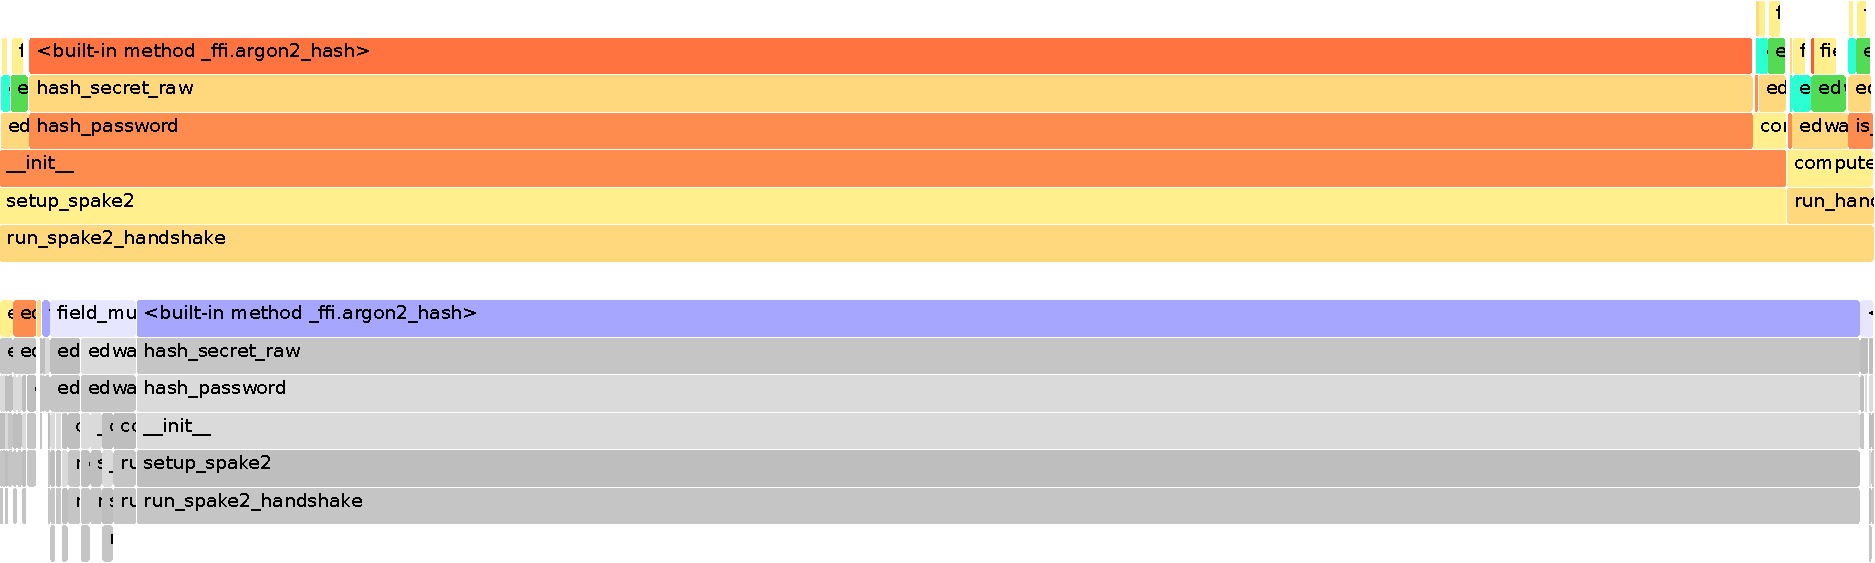
\includegraphics[width=0.8\linewidth]{Figs/spake2handshake.pdf} 
    \caption{Flamegraph of SPAKE2 Handshake Execution (Argon2 Overhead Highlighted)}
    \label{fig:spake2_flamegraph}
\end{figure}

\renewcommand{\thesection}{\Alph{section}}
\section{Profiling X25519 and Ed25519 Operations}
\label{sec:appendix_profiling}

This section presents the full benchmarking and profiling results for X25519 key exchange, Ed25519 signing, and Ed25519 verification. The profiling data was used to generate flame graphs to visualize function hotspots.

\subsection{Benchmark Results}

\begin{table}[h]
    \centering
    \renewcommand{\arraystretch}{1.2}
    \begin{tabular}{l c c c}
        \toprule
        \textbf{Metric} & \textbf{Ed25519 Signing} & \textbf{Ed25519 Verification} & \textbf{X25519 Key Exchange} \\
        \midrule
        Avg Time & 4.14 & 4.93 & 1.62 \\
        Median Time & 4.14 & 4.91 & 1.61 \\
        Std Deviation & 0.0168 & 0.0973 & 0.0225 \\
        Min Time & 4.11 & 4.85 & 1.60 \\
        Max Time & 4.16 & 5.10 & 1.65 \\
        P90 Latency & 4.16 & 5.17 & 1.67 \\
        P99 Latency & 4.16 & 5.27 & 1.69 \\
        \bottomrule
    \end{tabular}
    \caption{Ed25519 and X25519 Benchmark Results (Times in ms)}
    \label{tab:ed25519_x25519_benchmarks}
\end{table}

\subsection{Flame Graphs}

The following figures show flame graphs for each operation, highlighting where the most computation time is spent. As we can see in the figures, as well as in the profiling data, the \texttt{field\_mul} function is the main computational bottleneck in both X25519 and Ed25519 operations, particularly due to its repeated use in scalar multiplication and point operations.

\begin{figure}[h]
    \centering
    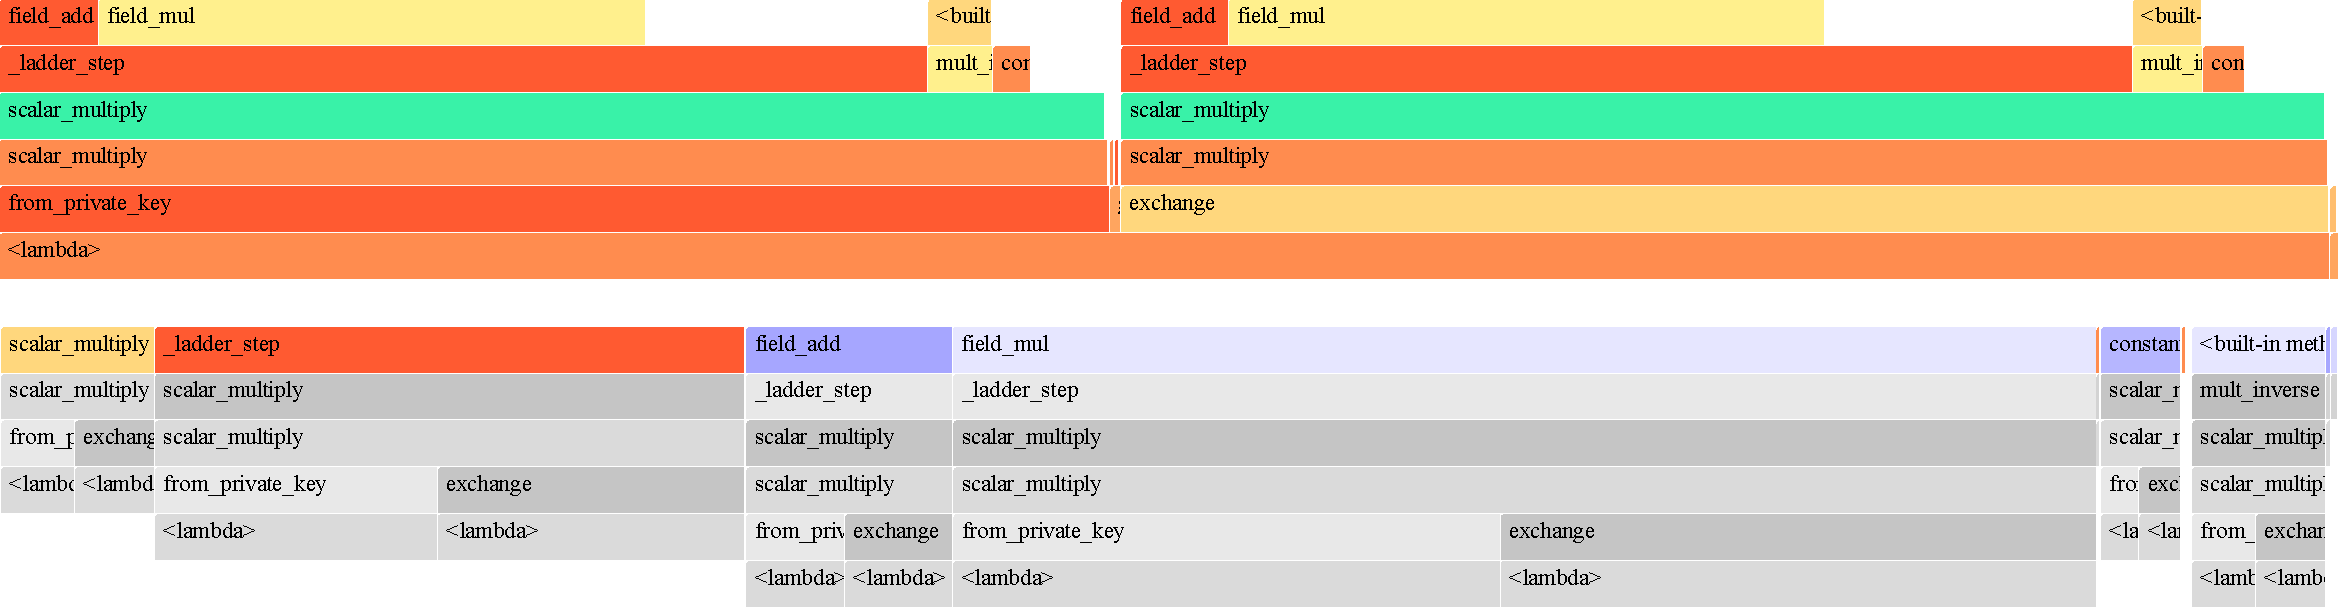
\includegraphics[width=0.8\textwidth]{Figs/x25519.pdf}
    \caption{Flame graph for X25519 key exchange}
    \label{fig:x25519_flamegraph}
\end{figure}

\begin{figure}[h]
    \centering
    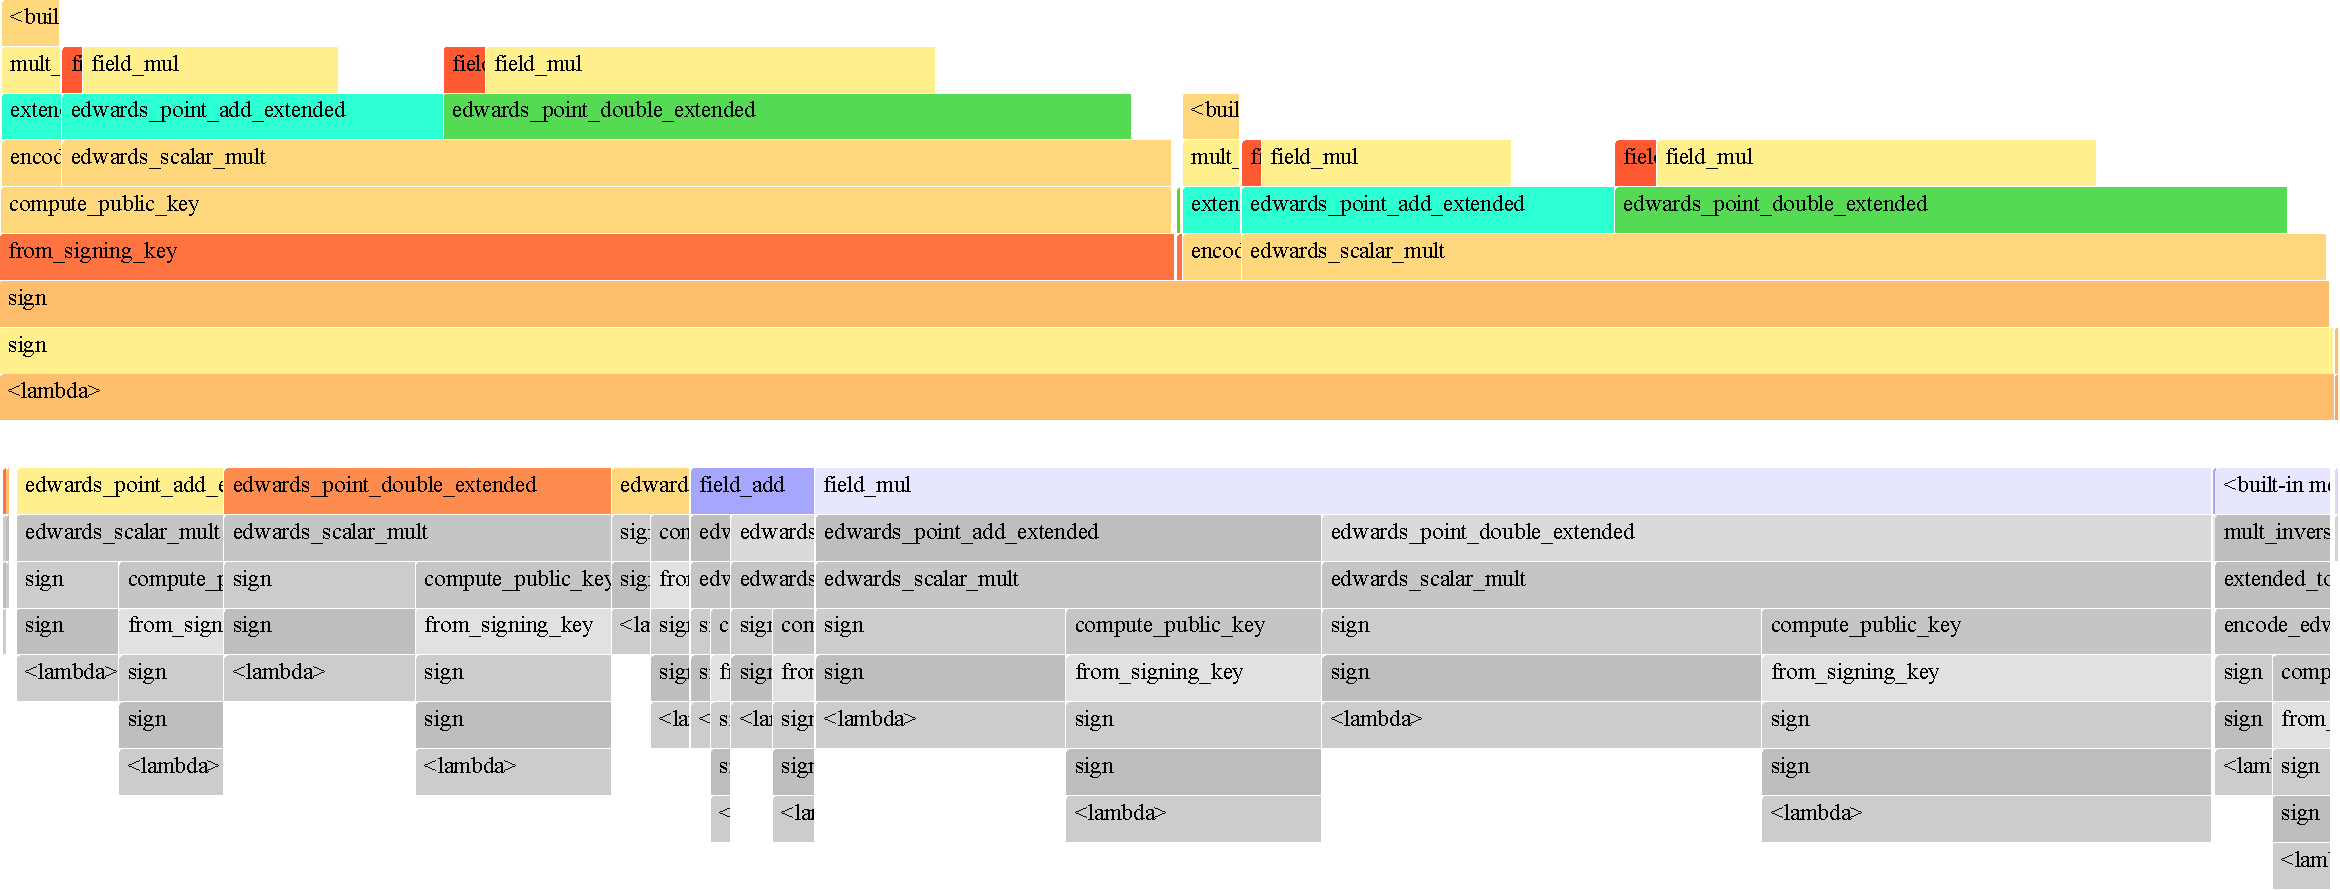
\includegraphics[width=0.8\textwidth]{Figs/ed25519sign.pdf}
    \caption{Flame graph for Ed25519 signing}
    \label{fig:ed25519_signing_flamegraph}
\end{figure}

\begin{figure}[h]
    \centering
    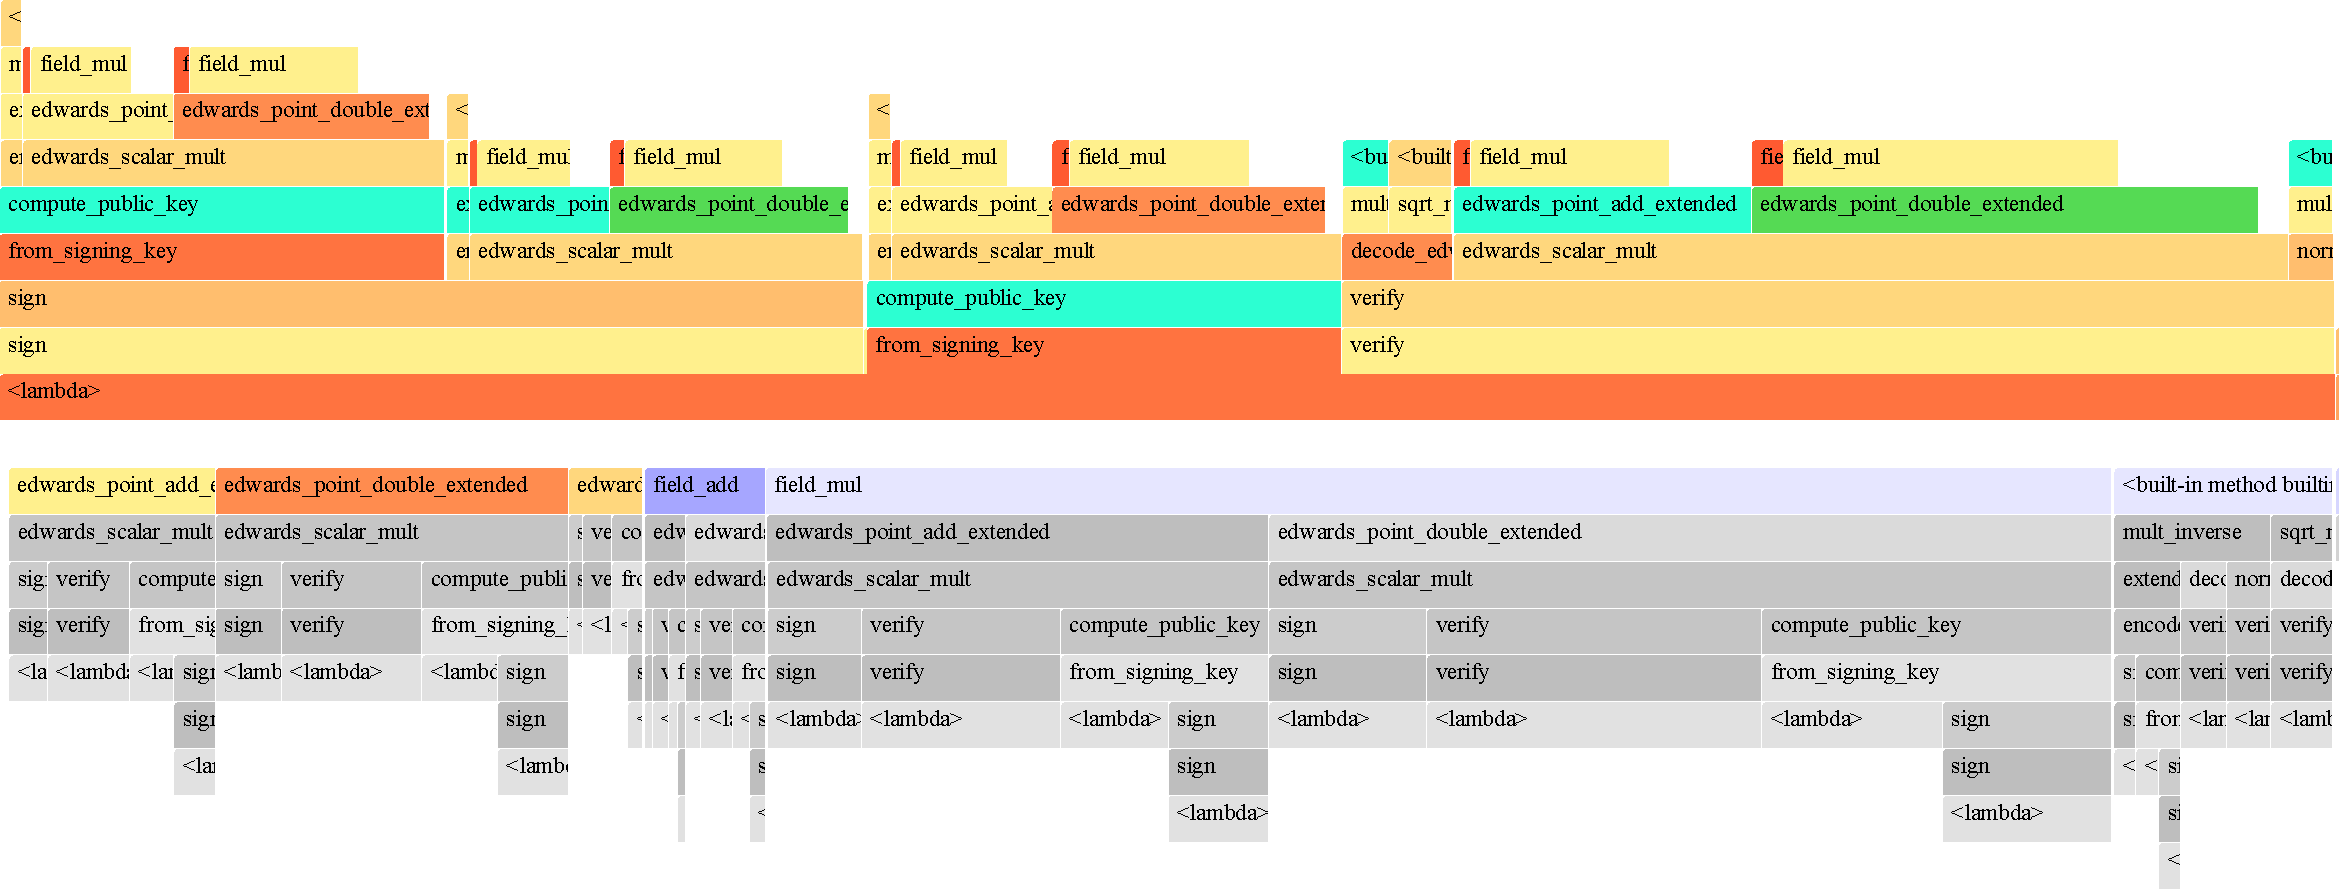
\includegraphics[width=0.8\textwidth]{Figs/ed25519verify.pdf}
    \caption{Flame graph for Ed25519 verification}
    \label{fig:ed25519_verification_flamegraph}
\end{figure}

%TC:endignore
\end{document}
